\chapter{State of the Art}

In the previous chapter, we introduced the basic idea of the tracking algorithm and the optimization methods. In this chapter, we first present more detailed knowledge of the implementation of the multitarget algorithm. In the first two sections, the basics of the traditional belt sorting system as well as the improvement in the \textit{TableSort}-System and the \textit{TrackSort} algorithm are presented. In Section 3.3, the implementation of the multitarget tracking algorithm is in detail explained, including the motion models used for tracking and the methods for data association and track management. Along these details, all the hyperparameters for optimizations in following chapters are listed.


\section{Overview of the Belt Sorting System}

Optical belt sorting is a versatile, state-of-the-art technology, which sorts bulk materials according to optical features. It usually comprises four parts: the feed system, the optical system, the data processing system, and the separation system, as illustrated in Figure \ref{belt sort system} \cite{edwards2004detecting}. The feed system usually consists of a material feeder and a conveyor belt or a slide, on which the materials flow through until being separated. This part can be also omitted, where the particles are in free fall before separation. The optical system contains cameras or sensors, which collect the location information of the material on the conveyor belt. The data processing system identifies the material and gives the prediction of the movement of the materials. Finally, the separation system separates the materials into different collectors.

\begin{figure}[htbp]
\centering
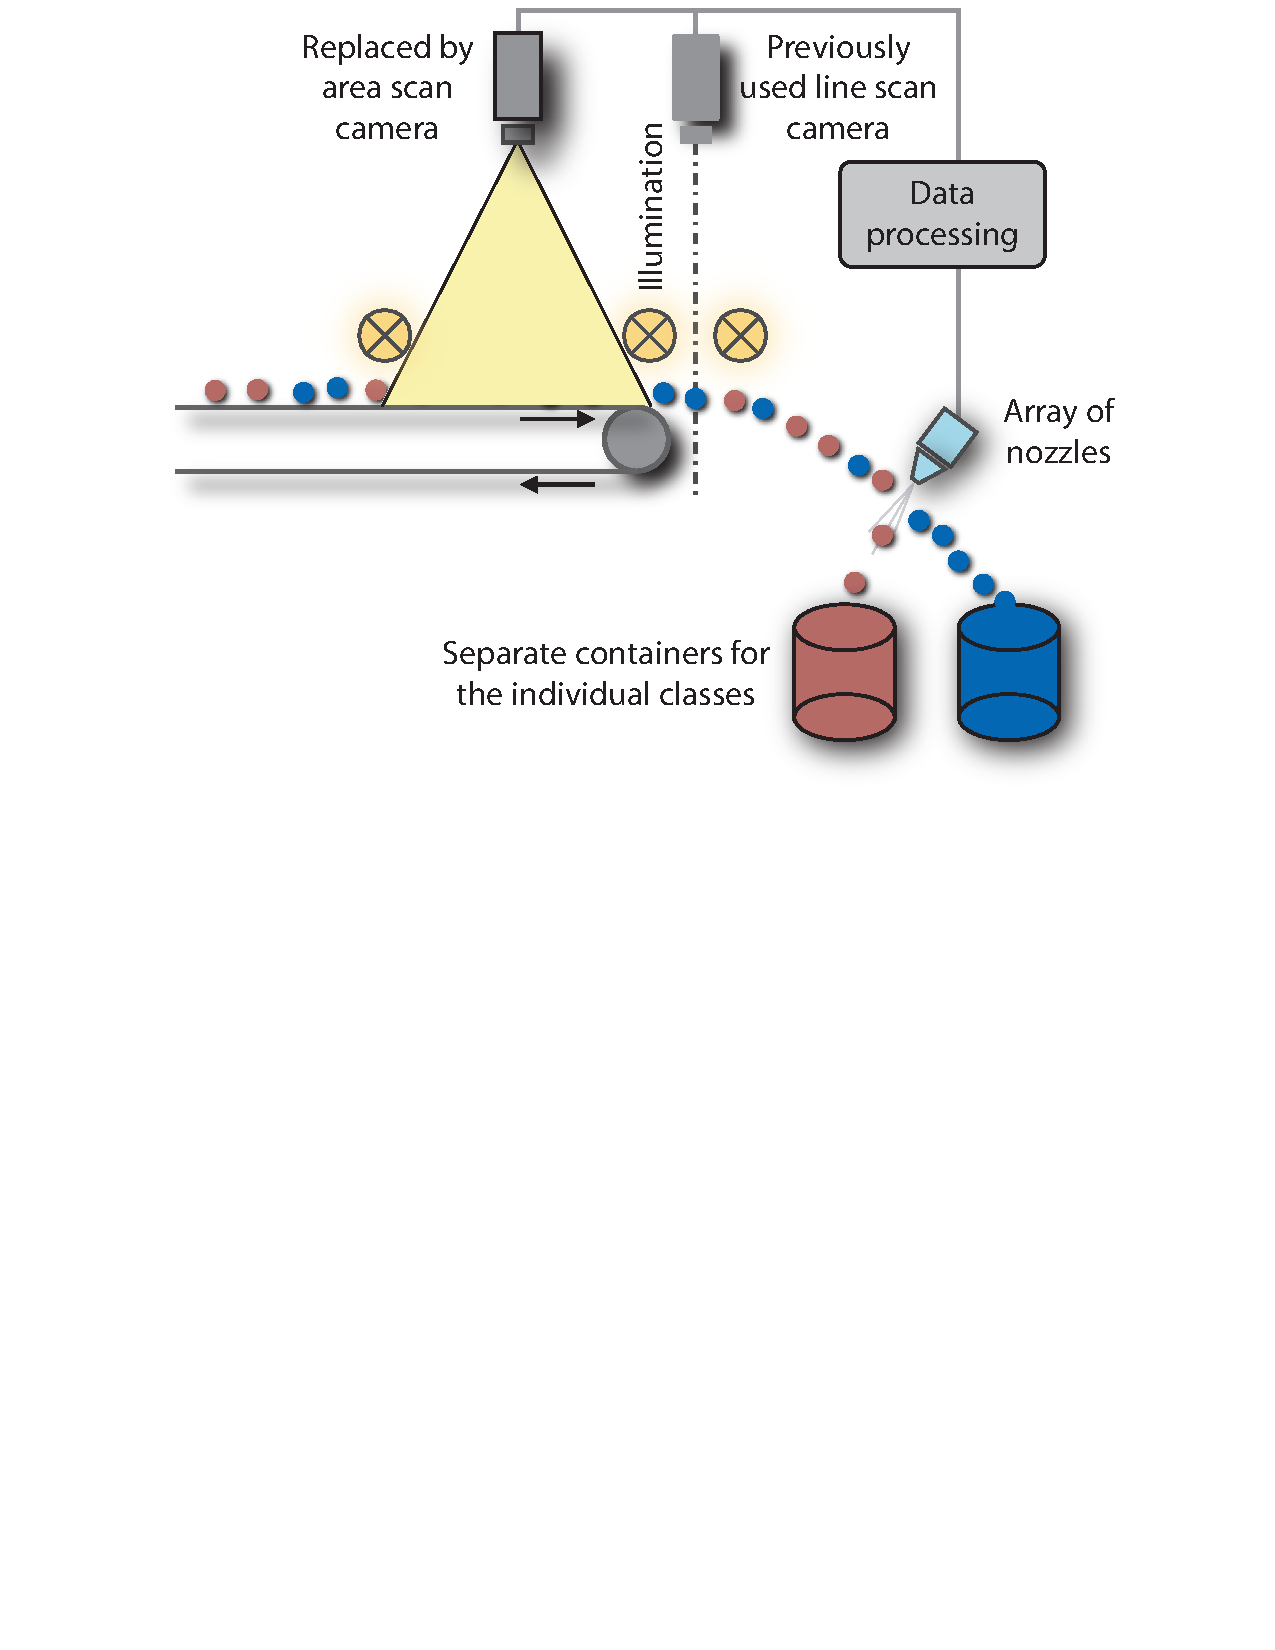
\includegraphics[width=0.6\textwidth]{figures/sort system.pdf}
\caption{Structure of a optical belt sorting system. In the recent research, the system with area scan camera has replaced the conventional system with line scan camera \cite{pfaff2017improving}.}
\label{belt sort system}
\end{figure}

The data processing system can be further divided into the image processing system, the tracking system and the prediction system. The image processing system transfers the image data from the camera into the particle centroid location and particle identity information. The tracking system tracks the movement of the particles in the tracking area and outputs the motion estimation of the particles. This part is also the main focus of this thesis. The prediction system predicts the time and location of the particles at the separator based on the information from the tracking system and certain motion models.
% \textcolor{red}{Add the traditional sorter here. The predictive sorting is moved to the next section.} 
Traditional optical belt sorters contain usually only line scan cameras or sensors, which observe the particles only once before the separator. As a result, traditional sorters can only gain a position measurement for each particle and can hardly do tracking on the particles. In the prediction system, because of the lack of the tracking information, the traditional optical belt sorters use the motion model that assumes the particles flying straightly in the transport direction without any motion orthogonal to the transport direction at a constant velocity, and the valve separator is activated after a fixed delay from detection of the particles. However, the particles do not always move straightly along the transport direction and may have a acceleration in flight. The motion model is not adequate for predicting such motion of the particles, which leads to a negative effect on tracking accuracy. 

\section{Introduction of \textit{TableSort} and \textit{TrackSort}}

The \textit{TableSort} system is a portable and flexible sorting platform, as shown in Figure \ref{fig:tablesortsystem}. One of the vital extensions of this system is to improve the separation results by utilization of the area scan camera and the predictive tracking method. The \textit{TableSort} system with the area scan camera can take several measurements for each particle in the tracking area and estimate the motion state of the particles. After the particles leave the tracking area, the predictive tracking algorithm can generate the predictions for the separation on the basis of the estimation from the tracking system and the motion model for the prediction part. This feature enables more accurate motion models in tracking and prediction.

\begin{figure}[htbp]
    \centering
	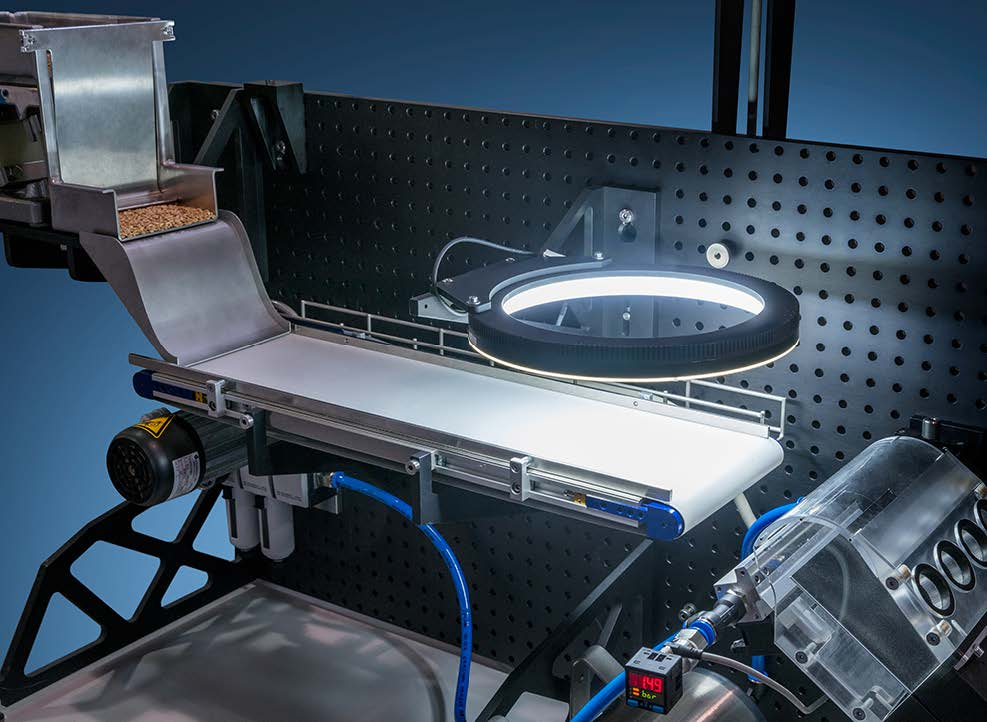
\includegraphics[width=0.8\textwidth]{figures/AT20-TrackSortMotionModels.jpg}
	\caption{Photo of \textit{TableSort} bulk material sorting system \cite{pfaff2020predictive}.}
	\label{fig:tablesortsystem}
\end{figure}

\section{Implementation of the \textit{TrackSort} Algorithm}

The \textit{TrackSort} algorithm developed by ISAS is used in the \textit{TableSort} system to estimate and predict the movement of each particle \cite{pfaff2015tracksort}. The process is divided into two phases. In the tracking phase, the position measurements on the belt are associated to each particle. With this position information, the motion of each particle is estimated by a recursive Kalman filter on the base of the motion model. This phase is the main focus of this thesis and will be further explained in the next section. After the particle has left the observation area of the camera, the algorithm enters into the prediction phase. The movement of the particles in this phase is predicted with the information from the tracking phase and the motion model, in order to determine an exact position and a time of separation. The motion models used in this phase are exhaustively introduced in \cite{pfaff2019multitarget}.

\subsection{Motion Models for Tracking}\label{Motion Models}

To balance the complexity and accuracy of the motion model, several assumptions are applied to different motion models. In belt sorting, we can assume that the material particles accelerate after touching the conveyor belt and then stay the same velocity with the belt. In this thesis, the constant velocity model (CV) and the constant velocity with angle model (CVA) are mainly used. Since the measurements are given in frame, only the discrete-time models are chosen.

\subsubsection{Constant Velocity Model}
% \textcolor{red}{Added the 2-D CV model.}

The constant velocity model is a widely used simple motion model for tracking particles that have entered a relatively stationary state with the belt. The 2-D CV model is used for the implementation of the tracking system. The noise terms in the motion model will be the hyperparameters for the sensitivity analysis and optimization.

In the 2-D constant velocity model, the state vector contains the position and velocity of the tracked objects along and vertical to the transport directions
\begin{equation}
    \underline{x}_{t}=
    \begin{bmatrix}
        \mathsf{x}_{t}\\ 
        \dot{\mathsf{x}}_{t}\\ 
        \mathsf{y}_{t}\\ 
        \dot{\mathsf{y}}_{t}
    \end{bmatrix}.
\end{equation}
Because the motion of the particles on different directions are considered as uncorrelated form each other, the system matrix for the constant velocity model is given as a block diagonal matrix with two system matrices from the 1-D CV model, as
\begin{equation}
    \mathbf{F}=\begin{bmatrix}
     1 & T & 0 & 0 \\ 
     0 & 1 & 0 & 0 \\ 
     0 & 0 & 1 & T \\ 
     0 & 0 & 0 & 1 
    \end{bmatrix}.
\end{equation}
In the implementation, the $T$ is always set as one, representing the time interval between each frame. Therefore, the time unit in this thesis will be frame.
The system noise covariance is also uncorrelated on different directions. Thus the matrix is given by
\begin{equation}
    \mathbf{C}^{\underline{\boldsymbol{w}}}=S^{\boldsymbol{w}}
    \begin{bmatrix}
     T^3/3 & T^2/2 & 0 & 0 \\ 
     T^2/2 & T     & 0 & 0 \\ 
     0 & 0 & T^3/3 & T^2/2 \\ 
     0 & 0 & T^2/2 & T 
    \end{bmatrix}.
\end{equation}
Only the position coordinates are directly observed in the measurement process. Therefore, the measurement matrix is
\begin{equation}
    \mathbf{H}=\begin{bmatrix}
     1 & 0 & 0 & 0 \\ 
     0 & 0 & 1 & 0 
    \end{bmatrix} .
\end{equation}
The measurement position covariance is a $2\times 2$ matrix. Because the measurement noise is generally uncorrelated on different directions and assumed to be same on different directions, it is given as the measurement variance multiplying an identical matrix, as
\begin{equation}
    \mathbf{C}^{\underline{\boldsymbol{v}}}= S^{\boldsymbol{v}}
    \begin{bmatrix}
     1 & 0 \\ 
     0 & 1
    \end{bmatrix} .
\end{equation}
Besides the parameters mentioned above, the initial parameters are also needed, as the initial position variance $S_{\mathrm{pos}}^{\mathrm{ini}}$, the initial velocity variance $S_{\mathrm{vel}}^{\mathrm{ini}}$ and the initial velocity guess $[\dot{\mathsf{x}}_{0}, \dot{\mathsf{y}}_{0}]$. In the implementation of  the \textit{TrackSort} algorithm, the initial variance is also assumed to be the same.  Therefore the initial estimated error covariance $\mathbf{C}_{0}^{\mathrm{e}}$ is given as
\begin{equation}
    \mathbf{C}^{\mathrm{e}}_{0}=
    \begin{bmatrix}
     S_{\mathrm{pos}}^{\mathrm{ini}} & 0 & 0 & 0 \\ 
     0 & S_{\mathrm{vel}}^{\mathrm{ini}} & 0 & 0 \\ 
     0 & 0 & S_{\mathrm{pos}}^{\mathrm{ini}} & 0 \\ 
     0 & 0 & 0 & S_{\mathrm{vel}}^{\mathrm{ini}}
    \end{bmatrix} .
\end{equation}
It is important to address that the initial velocity guess given from users is not always accurate. Therefore, when we have enough measurements, we use the average velocity calculated from measurements as the initial velocity guess for the initialization of new tracks instead. Because the initial velocity guess from measurements should be more close to the real initial velocity of the objects, the initial velocity variance should be lower. Therefore, the refined initial velocity variance $S_{\mathrm{vel}}^{\mathrm{ini, r}}$ is used after getting enough measurement data, which is different from the initial velocity variance $S_{\mathrm{vel}}^{\mathrm{ini}}$ used at the start of tracking. The hyperparameters in the CV model are listed in Table \ref{list hp cv}.
\begin{table}[htbp] 
    \centering
    \caption{List of hyperparameters for the CV model.} 
    \begin{tabular}{cc} 
    \toprule 
    Hyperparameters&Notation\\ 
    \midrule 
    Initial velocity guess              &$\underline{v}_{0}$\\
    Initial position variance           &$S_{\mathrm{pos}}^{\mathrm{ini}}$\\
    Initial velocity variance           &$S_{\mathrm{vel}}^{\mathrm{ini}}$\\
    Refined initial velocity variance   &$S_{\mathrm{vel}}^{\mathrm{ini, r}}$\\
    Measurement variance                &$S^{\boldsymbol{v}}$\\
    System noise variance               &$S^{\boldsymbol{w}}$\\ 
    \bottomrule 
    \end{tabular} 
    \label{list hp cv}
\end{table}

% Measurement noise density 

\subsubsection{Constant Velocity with Angle Model}

The constant velocity with angle model is similar to the constant velocity model, where the velocity of tracked objects are also considered as constant. However, the velocity of the tracked objects in the state vector of the CVA model is given with the magnitude of the velocity and the angle between the velocity and the transport direction. As a result, the state vector of this model contains the x- and y-coordinate of the object as well as the magnitude and the direction of the object velocity, as shown in Figure \ref{CVA}
\begin{equation}
    \underline{x}_{t}=
    \begin{bmatrix}
        \mathsf{x}_{t}\\ 
        \mathsf{y}_{t}\\ 
        \mathsf{v}_{t}\\ 
        \theta_{t}
    \end{bmatrix}.
\end{equation}
\begin{figure}[htbp]
	\centering
	\begin{subfigure}[t]{0.49\textwidth}
		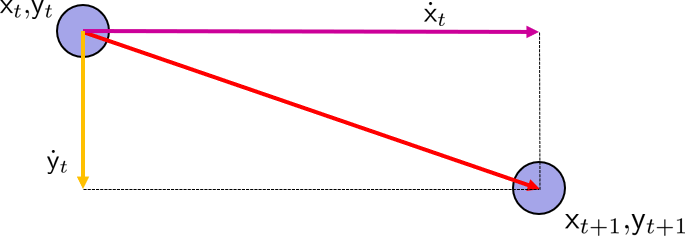
\includegraphics[width=\textwidth]{figures/CVmodel.png}
		\caption{CV model}
	\end{subfigure}
% 	\vskip\baselineskip
	\begin{subfigure}[t]{0.49\textwidth}
		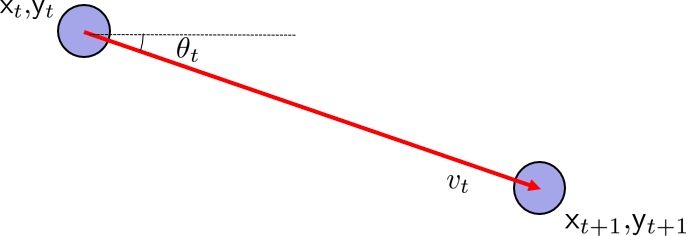
\includegraphics[width=\textwidth]{figures/CVAmodel.png}
		\caption{CVA model}
		\label{CVA}
	\end{subfigure}
	\caption{The illustration of the two motion models in this thesis.}
	\label{motion model}
\end{figure}
The relationship between state variables in the constant velocity model is not linear. Therefore, the predict and update processes of different state variables are done in three separated Kalman filter, and the variances for different state variables are also given separately. 

In the prediction step, the state transition function of the x- and y-coordinate of the object is given as
\begin{equation}
    \begin{bmatrix}
    \mathsf{x}_{t}^{\mathrm{p}}\\
    \mathsf{y}_{t}^{\mathrm{p}}\\
    \end{bmatrix}
    =
    \begin{bmatrix}
    \mathsf{x}_{t-1}^{\mathrm{e}}\\
    \mathsf{y}_{t-1}^{\mathrm{e}}\\
    \end{bmatrix}
    +
    \begin{bmatrix}
    \mathsf{v}_{t-1}^{\mathrm{e}}\cos\theta_{t}^{\mathrm{e}}\\
    \mathsf{v}_{t-1}^{\mathrm{e}}\sin\theta_{t}^{\mathrm{e}}\\
    \end{bmatrix}.
\end{equation}
The magnitude of the velocity and the angle between the velocity and the transport direction stay unchanged in the prediction step. The covariance for the position as well as the variance for the velocity magnitude and angle all follow the equation
\begin{equation}
    S_{t}^{\mathrm{p}}=S_{t-1}^{\mathrm{e}}+S^{\boldsymbol{w}}.
\end{equation}
% \begin{gather}
%     \mathbf{F}_{\mathsf{x},\mathsf{x}}=\begin{bmatrix}
%      1 & 0 & T\cos\theta & 0 \\ 
%      0 & 1 & T\sin\theta & 0 \\ 
%      0 & 0 & 1 & 0 \\ 
%      0 & 0 & 0 & 1 
%     \end{bmatrix} ,\\
%     \mathbf{C}^{\underline{\boldsymbol{w}}}=
%     \begin{bmatrix}
%      S_{\mathrm{pos}}^{\underline{\boldsymbol{w}}} & 0 & 0 & 0 \\ 
%      0 & S_{\mathrm{pos}}^{\underline{\boldsymbol{w}}} & 0 & 0 \\ 
%      0 & 0 & S_{\mathrm{vel}}^{\underline{\boldsymbol{w}}} & 0 \\ 
%      0 & 0 & 0 & S_{\mathrm{ang}}^{\underline{\boldsymbol{w}}}
%     \end{bmatrix} .
% \end{gather}
In the constant velocity with angle model, the position can be directly extracted from each frame of the measurement. The measurement value of the velocity magnitude and the angle are derived from the predicted position of this timestep and the updated position of last timestep, as
\begin{gather}
    \mathsf{v}_{t}^{\mathrm{m}}=\sqrt{(\mathsf{x}_{t}^{\mathrm{p}}-\mathsf{x}_{t-1}^{\mathrm{e}})^{2}+(\mathsf{y}_{t}^{\mathrm{p}}-\mathsf{y}_{t-1}^{\mathrm{e}})^{2}},\\
    \theta_{t}^{\mathrm{m}}=\arctan(\frac{\mathsf{y}_{t}^{\mathrm{p}}-\mathsf{y}_{t-1}^{\mathrm{e}}}{\mathsf{x}_{t}^{\mathrm{p}}-\mathsf{x}_{t-1}^{\mathrm{e}}}).
\end{gather}
The update equations are given as
\begin{gather}
    x^{\mathrm{e}}_{t}=\frac{{S_{t}^{\mathrm{p}}}^{-1}+{S^{\boldsymbol{v}}}^{-1}}{\frac{S_{t}^{\mathrm{p}}}{x_{t}^{\mathrm{p}}}+\frac{S^{\underline{\boldsymbol{v}}}}{x_{t}^{\mathrm{m}}}},\\
    S_{t}^{\mathrm{e}}=({{S_{t}^{\mathrm{p}}}^{-1}+{S^{\boldsymbol{v}}}^{-1}})^{-1},
\end{gather}
where the $x$ represents the state variables and $S$ represents the variance or covariance of them.

\begin{table}[htbp] 
    \centering
    \caption{List of hyperparameters for the CVA model.} 
    \begin{tabular}{cc} 
    \toprule 
    Hyperparameters&Notation\\ 
    \midrule 
    Initial velocity guess&$v_{0}$\\
    Initial angle guess&$\theta_{0}$\\
    Initial position variance         &$S_{\mathrm{pos}}^{\mathrm{ini}}$\\
    Initial velocity variance           &$S_{\mathrm{vel}}^{\mathrm{ini}}$\\
    Refined initial velocity variance&$S_{\mathrm{vel}}^{\mathrm{ini, r}}$\\
    Initial angle variance          &$S_{\mathrm{ang}}^{\mathrm{ini}}$\\
    Measurement position variance   &$S_{\mathrm{pos}}^{\boldsymbol{v}}$\\
    Measurement velocity variance   &$S_{\mathrm{vel}}^{\boldsymbol{v}}$\\
    Measurement angle variance      &$S_{\mathrm{ang}}^{\boldsymbol{v}}$\\
    Prediction position variance    &$S_{\mathrm{pos}}^{\boldsymbol{w}}$\\
    Prediction velocity variance    &$S_{\mathrm{vel}}^{\boldsymbol{w}}$\\
    Prediction angle variance       &$S_{\mathrm{ang}}^{\boldsymbol{w}}$\\
    \bottomrule 
    \end{tabular} 
    \label{list HP cva}
\end{table}

Which is identical to the CV model, the initial parameters are also needed in the CVA model. The initial estimated error covariance for position, velocity magnitude and angle are given separately. The refined initial velocity variance $S_{\mathrm{vel}}^{\mathrm{ini, r}}$ is still given a different value from the initial velocity variance $S_{\mathrm{vel}}^{\mathrm{ini}}$. The list of the hyperparameters for the CVA model is presented in Table \ref{list HP cva}.

\subsection{Data Association}
\label{Data Association soa}

% \textcolor{red}{todo: move some thing here}
% \textcolor{red}{todo: rewrite here. What the intuition behind the association matrix? What does it contain? Formulas would greatly help to understand the section better.}

In the data association process, each new observed measurement is assigned to a corresponding track. The likelihood for a measurement $\underline{\hat{z}}$ associated from the $i$th track is defined as $\ell(\underline{\hat{z}}|i)$. When we have $n$ measurements and $n$ tracks, the association can be seen as a permutation $\tau$ of ${1,...,n}$. In this case, the likelihood of the whole association is 
\begin{equation}
    \ell(\underline{\hat{z}}^{\tau(1)},\underline{\hat{z}}^{\tau(2)},...,\underline{\hat{z}}^{\tau(n)}|1,2,...,n)=\prod_{i=1}^{n}\ell(\underline{\hat{z}}^{\tau(i)}|i).
\end{equation}

The association process maximizes this likelihood. \cite{pfaff2019multitarget} shows that the negative log of the likelihood can be represent with 
\begin{equation}
\begin{aligned}
    \label{likelihood}
    &-\log\ell(\underline{\hat{z}}^{\tau(1)},\underline{\hat{z}}^{\tau(2)},...,\underline{\hat{z}}^{\tau(n)}|1,2,...,n)\\
    =&\frac{1}{2}\sum_{i=1}^{n}\log \left (\det 2 \pi(\textbf{H}\textbf{C}^{\mathrm{p},i}\textbf{H}^\top+\mathbf{C}^{\underline{\boldsymbol{v}}})\right )\\
    &+\frac{1}{2}\sum_{i=1}^{n}\left ( \underset{\text{Squared Mahalanobis distance}}{\underbrace{(\underline{\hat{z}}^{\tau(i)}-\textbf{H}\underline{\hat{x}}^{\mathrm{p},i})^\top(\textbf{H}\textbf{C}^{\mathrm{p},i}\textbf{H}^\top+\mathbf{C}^{\underline{\boldsymbol{v}}})^{-1}(\underline{\hat{z}}^{\tau(i)}-\textbf{H}\underline{\hat{x}}^{\mathrm{p},i})}} \right ).
\end{aligned}
\end{equation}

Therefore, the squared Mahalanobis distances can represent the association likelihoods, and minimizing the summation of the squared Mahalanobis distances from all measurement-track pairs can maximize the likelihood of the association. In this case, we use the association matrix filled with the squared Mahalanobis distance between each measurement and predictions for the association work. The GNN solves the linear assignment problem (LAP) of the association matrix with minimizing the sum of the values from all selected cells. The association results are represented with the selection of the blocks in the matrix, and the summation of the numbers in the selected blocks should be smallest among all possible associations.

\begin{figure}[htb]
\centering
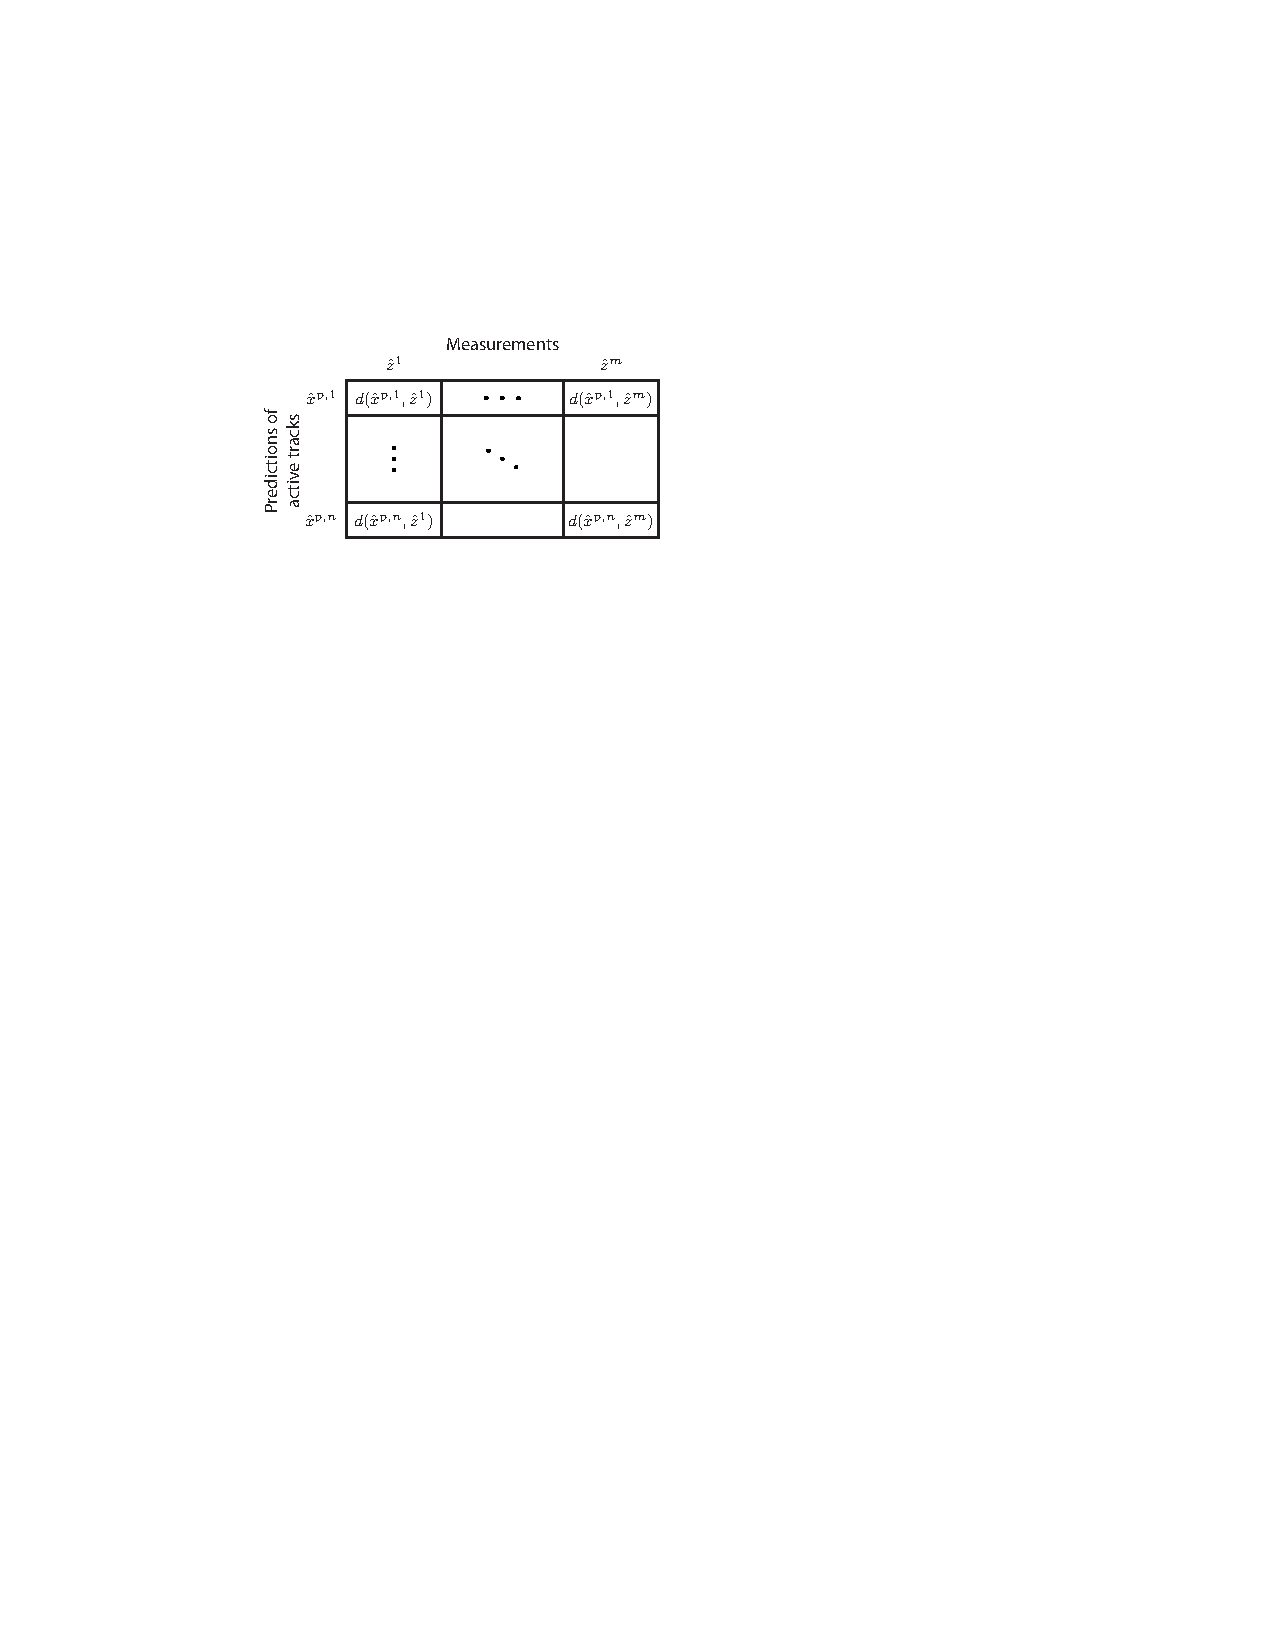
\includegraphics[width=0.6\textwidth]{figures/asso matrix small.pdf}
\caption{Matrix used for the determination of the association decisions. The value in each block is the squared Mahalanobis distance between a measurement and a prediction \cite{pfaff2019multitarget}.}
\label{association matrix simple}
\end{figure}



\subsection{Track Management}

In the optical sorting tasks, particles appear at the start of the observation area and disappear at end start of the observation area. According to \cite{mahler2007statistical}, we can define three states of a track. The first one is \textit{existing} that means a track is extending in the tracking area and should be assigned with a measurement. All the tracks in Figure \ref{association matrix simple} belong to this state. The second one is \textit{appearing} that represents a track is first observed in this timestep. In this case, the new measurement is not assigned to a existing track and should be used for the initialization of the new track. The last one is \textit{disappearing} that means a track is extending out of the tracking area. No measurements is assigned to a disappearing track.

In order to deal with the appearing and disappearing tracks, the extended association matrix is used in the association algorithm, as illustrated in Figure \ref{association matrix}. Except for the cells filled with squared Mahalanobis distances that indicate the distance between each measurement and prediction same as in Figure \ref{association matrix simple}, the other cells of the extended association matrix are filled with distance-like penalty terms that showing the likelihoods of the tracks appearing and disappearing. In this thesis, the association problem is also solved with the GNN \cite{pfaff2019multitarget}. As mentioned in Equation \eqref{likelihood}, it means the likelihood of the association decision from the GNN is maximized. The associated track–measurement pairs can be represented with the indices of the selected cells in the association matrix.



\begin{figure}[htb]
\centering
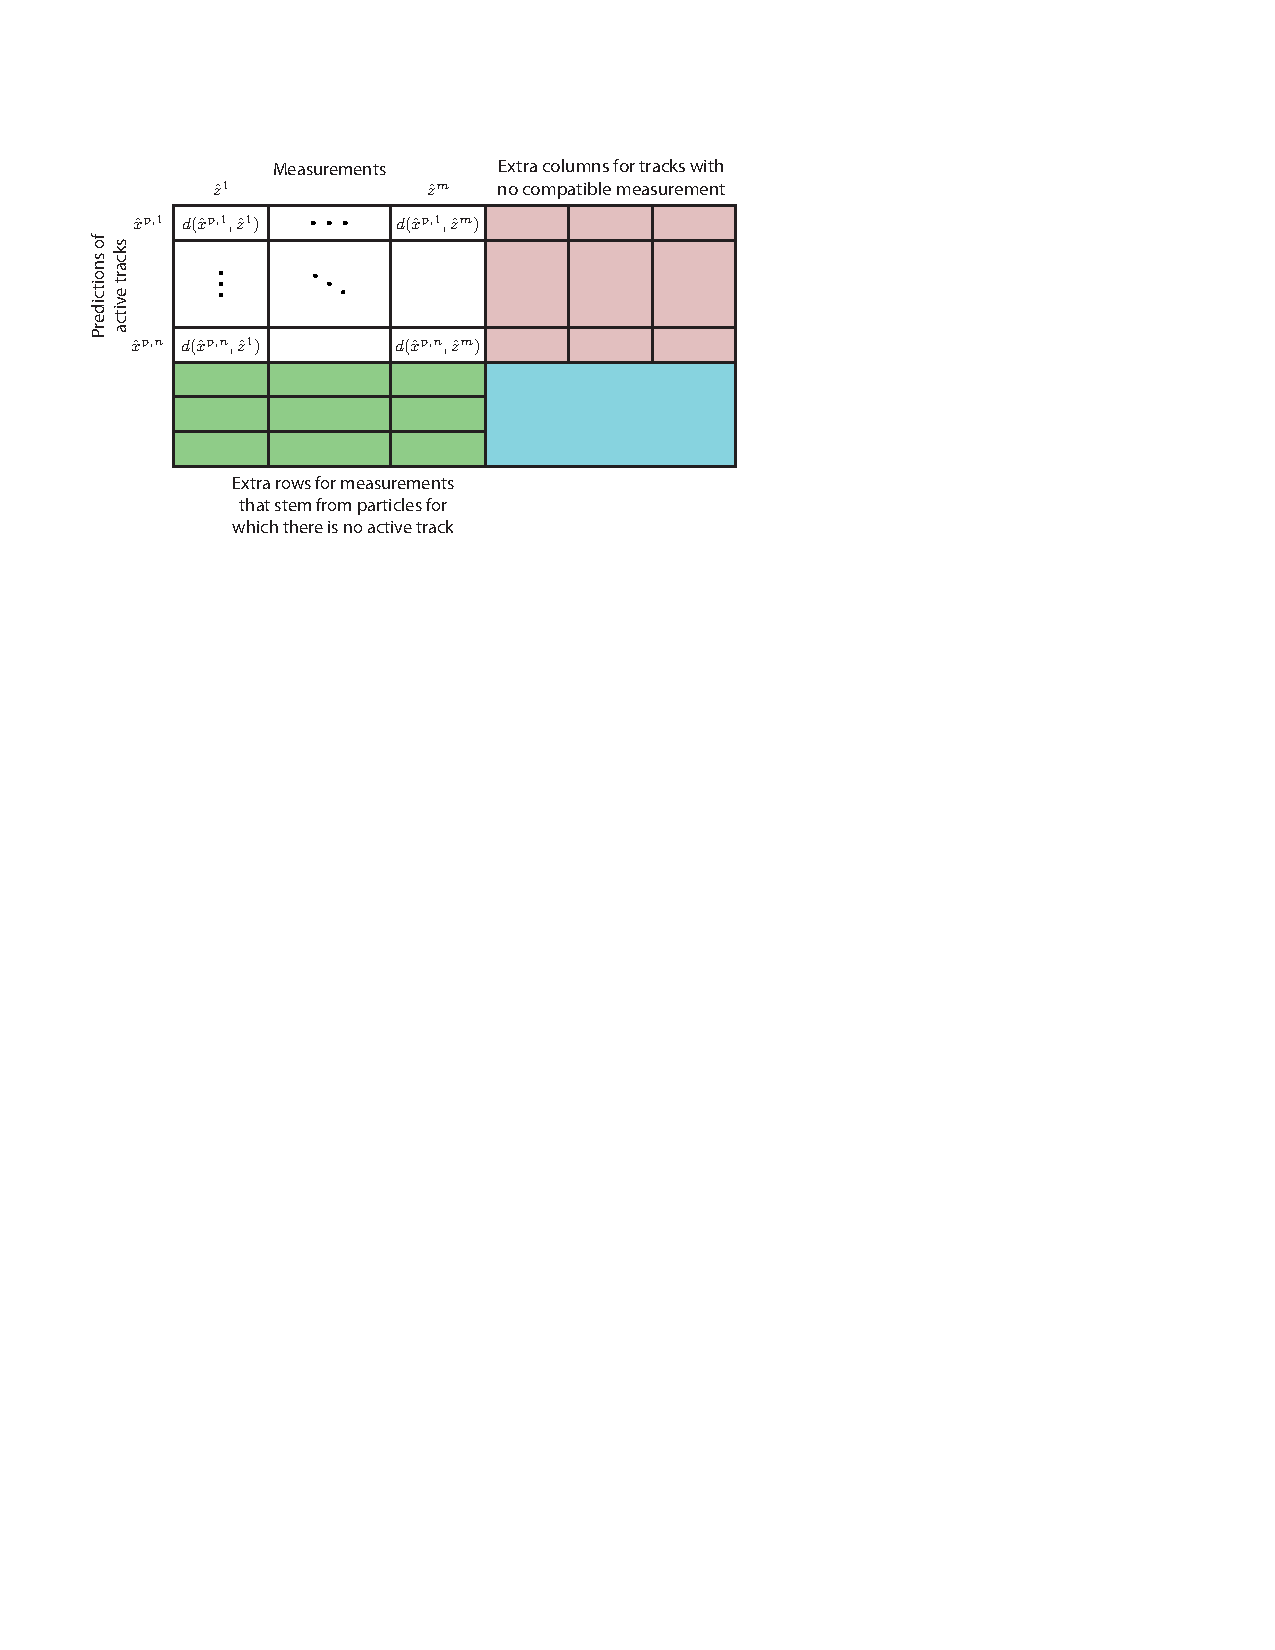
\includegraphics[width=0.8\textwidth]{figures/asso matrix.pdf}
\caption{The extended association matrix used in the implementation of the multitarget tracking algorithm. The areas with different colors represents different state of measurements and tracks \cite{pfaff2019multitarget}.}
\label{association matrix}
\end{figure}


The upper left area includes the squared Mahalanobis distance between each measurement and prediction. When the blocks appear in the result of the LAP, the corresponding measurements are assigned to existed tracks. The size of the upper left area is $m\times n$, where $m$ is the number of active tracks and $n$ is the number of measurements. 
% This area is filled with the squared Mahalanobis distance between each new measurements and predictions of active tracks, as suggested in Equation \eqref{likelihood}.

If the blocks from the upper right area and the bottom left area appear in the result of the LAP, it means respectively the cases of tracks disappearing or appearing. The number of extra columns and rows can be set manually. When this number is higher, the tracking system can deal with more newly appearing tracks. However, using more columns and rows than necessary will cause higher run times, since the problem size of the LAP is larger. 

These two areas dealing appearing and disappearing tracks are filled with distance-like penalty terms. These penalty values represent the probabilities for track appearing and disappearing. When these penalty terms are lower, the tracks or measurements are more possible in this state. In other words, the corresponding cells are more easily to be chosen in the association decision from the GNN algorithm. However, the probabilities for track appearing and disappearing vary at different parts of the belt, as illustrated in Figure \ref{association along belt}. For example, tracks are more possible to appear at the start of the tracking area, but less possible to appear in the middle. Therefore, the value of penalty terms should be a function of the position in the tracking area. In this thesis, the different values of penalty terms are realized with a step function, which gives different penalty terms at different parts of the tracking area. Therefore, two values for penalty terms of track appearing and two for track disappearing are needed. In order to fit the values in the upper right area, the value of those terms should change with different tracking settings, such as belt velocity, particle density on the belt and the noise level in the tracking. The boundary of different tracking area is determined by the product of the initial velocity guess and the additional safety margin coefficient, which are also the hyperparameters in this thesis.

The cells in the blue area in Figure \ref{association matrix} are also filled with penalty terms. The cells in this area are included in the association decision when the extra rows or columns are more than necessary. This probability is not related to the tracking area, so the penalty term here remains the same in the tracking. All the penalty terms as well as the boundary between different tracking phases are considered as hyperparameters in this thesis. These association hyperparameters are listed in Table \ref{List of association hyperparameters}. 

% \textcolor{red}{I have read a document stating that all quantities and variables should be in italic and all units and descriptive terms should be in roman, so I changed all subscripts in the table below into roman even if there is only one letter, like $d_{\mathrm{n}}$}

% \textcolor{red}{This paragraph is small, but also has no relation to the other paragraphs, so it seems strange to merge it into other paragraphs.}

\begin{table}[htbp] 
\small
    \centering
    \caption{List of association hyperparameters.} 
    \label{List of association hyperparameters}
    \begin{tabular}{ccc} 
    \toprule 
    Hyperparameters&Notation&Use\\ 
    \midrule 
    Distance appear at start &$d_{\mathrm{as}}$&For green blocks in Figure \ref{association matrix} in the start phase\\
    Distance appear at middle &$d_{\mathrm{am}}$&For green blocks in Figure \ref{association matrix} in the other phases\\
    Distance disappear at end &$d_{\mathrm{de}}$&For red blocks in Figure \ref{association matrix} in the end phase\\
    Distance disappear at middle &$d_{\mathrm{dm}}$&For red blocks in Figure \ref{association matrix} in the other phases\\
    Distance no change &$d_{\mathrm{n}}$&For blue blocks in Figure \ref{association matrix}\\
    \multirow{2}*{Starting phase coefficient}&\multirow{2}*{$l_{\mathrm{s}}$}& The coefficient determining the boundary\\
    &&between starting and middle phase\\
    \multirow{2}*{Ending phase coefficient}&\multirow{2}*{$l_{\mathrm{e}}$}& The coefficient determining the boundary\\
    &&between middle and end phase\\
    \bottomrule 
    \end{tabular} 
\end{table}

\begin{figure}[htb]
\centering
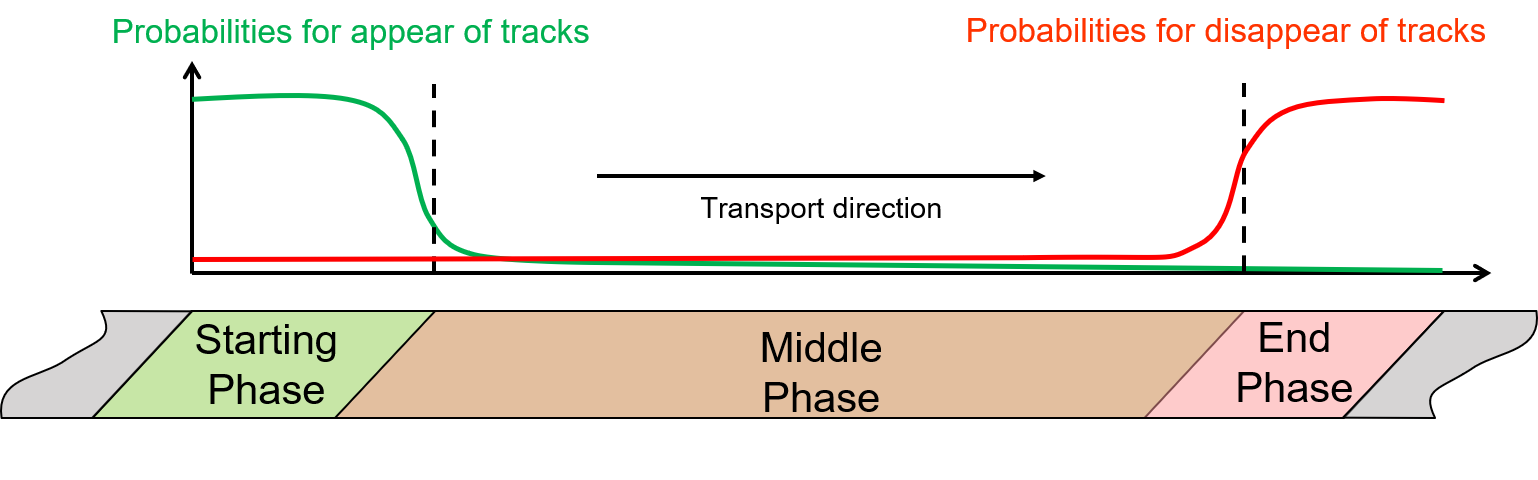
\includegraphics[width=0.8\textwidth]{figures/association along belt.png}
\caption{Probabilities that a new track observed or a track disappeared, adapted from \cite{pfaff2019multitarget}.}
\label{association along belt}
\end{figure}


The appearing tracks from the data association phase need to be initialized for the prediction of the next timestep. In both motion models mentioned in \Sec{Motion Models}, the initial position is initialized as the new measurement. The initial velocity along the transport direction is determined with the initial guess provided by the user at the start of the tracking process. Since this guess is only an inaccurate guess of the initial velocity, this guess is only used in the start of tracking and accompanied with a high variance. After having enough measurements, the initial velocity is refined with the average velocity of the observed particles in every timestep. The list of the initial variances are presented in \Tab{list hp cv} and \ref{list HP cva}. 
% These values can have an effect on tracking accuracy.

Because of errors in image processing, particles can be missed in some timesteps, and the tracks can be interrupted in the middle of the tracking area. To reduce this error, track scores are introduced in the tracking algorithm. Each new track is initialized with a start track score. When the track is associated with a measurement, the track extends normally and the track score increases. When the track has no measurement associated, the track is not regarded as ended immediately, but the track score decreases. Only until the track score is less than a threshold, the track is considered as ended and no longer participate the association .

Until now, we have figured out all the hyperparameters we need to optimize and summarized all the optimization and classification methods we need. In following chapters, we will introduce the operation details of the optimization, including the dataset we use, the configuration of the optimization methods and the optimization results.





























